%%%%%%%%%%%%%%%%%%%%%%%%%%%%%%%%%%%%%%%%%%%%%%%%%%%%%%%%%%%%%%%%%%%%%%%
%%  Indoor-Navigation mit Smartphone-Sensorik                        %%
%%-------------------------------------------------------------------%%
%% Datei:        101_introduction.tex                                %%
%% Beschreibung: Titelseite für die Abschlussarbeit                  %%
%% Autor:        Maximilian Helfrich                                 %%
%% Datum:        01.05.2021                                          %%
%% Version:      1.0.0                                               %%
%%%%%%%%%%%%%%%%%%%%%%%%%%%%%%%%%%%%%%%%%%%%%%%%%%%%%%%%%%%%%%%%%%%%%%%
\chapter{Anleitung} \index{Anleitung}

Diese Anleitung bietet einen Überblick über das Template für Bachelorarbeiten im Institut etti 6, und ist selbst ein Beispiel für die Anwendung Dieser. 

\section{Titelblatt und Erklärung}\index{Titelblatt und Erklärung}\label{Titelblatt und Erklärung}

Das Titelblatt und die Erklärung sind bereits erstellt, und die Quelldateien müssen nicht mehr angepasst werden. Die Belegung der Variablen für Name, Datum, etc. findet im Einstiegspunkt, der Datei thesis.tex statt. Die zu ändernden Variablen sind durch Kommentare markiert.

\section{Abstract}\index{Abstract}\label{Abstract}

Standardmäßig wird in diesem Template ein Abstract erzeugt. Sollte dies nicht gewünscht sein, kann die Erzeugung des Abstract in der Datei thesis.tex durch auskommentieren deaktiviert werden. Der Text des Abstract kann in der Datei source\slash002\textunderscore abstract.tex angepasst werden.

\section{Inhaltsverzeichnis}\index{Inhaltsverzeichnis}\label{Inhaltsverzeichnis}

Das Inhaltsverzeichnis wird automatisch erzeugt. Die Tiefe kann in der Datei thesis.tex angepasst werden.

\section{Hauptteil}\index{Hauptteil}\label{Hauptteil}

Es bietet sich an, für jedes Kapitel eine eigene .tex-Datei im source-Ordner zu erzeugen. Um diese einzubinden, müssen sie in der Datei thesis.tex referenziert werden.

\begin{figure}[H]
    \centering
    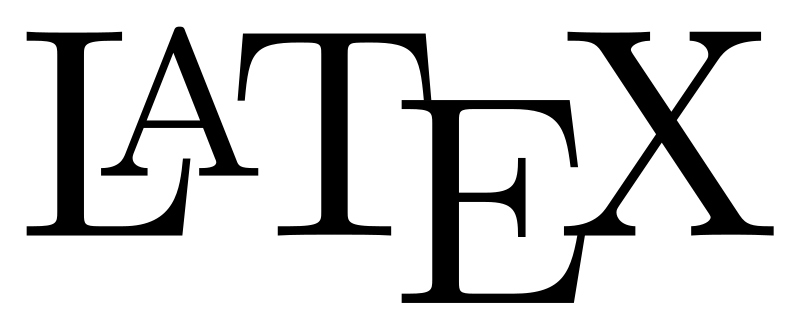
\includegraphics[width={\textwidth/2}]{images/pictures/LaTeX_logo.svg.png}
    \caption{Beispielabbildung}
    \label{figure:example}
\end{figure}

\section{Anhang}\index{Anhang}\label{Anhang}

\subsection{Abbildungen}\index{Abbildungen}\label{Abbildungen}

Das Abbildungsverzeichnis wird automatisch erstellt, als Beispiel hierfür dient die oben gezeigte Beispielabbildung. Dies kann verhindert werden, indem die entsprechende Anweisung in der Datei 801\textunderscore appendix.tex auskommentiert wird.

\subsection{Abkürzungen und Glossar}\index{Abkürzungen und Glossar}\label{Abkürzungen und Glossar}

Abkürzungen wie etwa \acrshort{ba} und Erläuterungen wie \Gls{latex}-Template können in der Datei acronym.tex ergänzt werden. Die entsprechenden Verzeichnisse im Anhang werden automatisch erzeugt.


\subsection{Quellcode}\index{Quellcode}\label{Quellcode}
{\setstretch{1}
\lstinputlisting[
    style=Java, 
    language=c, 
    caption={thesis.js}
    \label{lst:jsThesis}
]{code/thesis.js}
}\index{thesis.js}

\subsection{Literaturverzeichnis}\index{Literaturverzeichnis}\label{Literaturverzeichnis}
Das Literaturverzeichnis wird automatisch erstellt. Dafür wird eine Literaturdatenbank (Dateiformat .bib) benötigt. Empfehlenswert hierfür sind die Programme Zitavi (Windows) oder Zotero (MacOs / Linux). Aus diesen können diese erzeugten Bibliotheken exportiert, und in die oberste Ebene der Ordnerstruktur des Templates unter dem Namen Literatur.bib eingefügt werden. Zitate, die im Text vorkommen, werden automatisch in das Literaturverzeichnis übernommen.
Kennzeichnen von indirekten Zitaten \cite{noauthor_software_nodate}, und "direkten Zitaten" \cite[s.~234]{noauthor_software_nodate} erzeugt somit dem IEEE-Zitierstil entsprechenden Zitate.
\newpage

\subsection{Tabellenverzeichnis}\index{Tabellenverzeichnis}\label{Tabellenverzeichnis}
Das Tabellenverzeichnis wird automatosch erstellt, wie die Folgende Beispieltablle zeigt:

\begin{table}[h!]
\centering
 \begin{tabular}{||c c c c||} 
 \hline
 a & b & c & d \\ [0.5ex] 
 \hline\hline
 1 & 6 & 11 & 16 \\ 
 2 & 7 & 12 & 17 \\
 3 & 8 & 13 & 18 \\
 4 & 9 & 14 & 19 \\
 5 & 10 & 15 & 20 \\ [1ex] 
 \hline
 \end{tabular}
 \caption{Beispieltabelle}
\end{table}

\chapter{Einleitung}\index{Einleitung}
In der modernen Zeit der Digitalisierung spielt die effiziente und effektive Verarbeitung von Daten eine entscheidende Rolle. Dabei stellt sich auch die Frage, wie Datensätze am besten dargestellt werden können, um die richtigen Informationen leicht erkennbar zu machen. Neben den bekannten Formen wie Balken-, Kreis- oder Liniendiagrammen besteht in der Informatik auch die Möglichkeit, Datensätze in Form eines Graphen zu präsentieren.

\section{Hintergrund und Motivation}\index{Hintergrund und Motivation}\label{Hintergrund und Motivation}
In einer Projektarbeit, welcher dieser Bachelorarbeit vorangegangen ist, habe ich mich mit der Aufgabe beschäftigt kleine Gruppen von Profifussballspielern in  einem kompletten Graph zu entdecken, welche häufig zusammen den Verein wechseln. Bei dieser Aufgabe wurden qualitativ leider keine guten Ergebnisse generiert, worauf hin sich folgende Fragestellung  entwickelte, mit der ich mich in dieser wissenschaftlichen Arbeit beschäftigen will. Wie können Community Detection Algorithmen effektiv und effizient angewendet werden um optimale Ergebnisse zu erzielen, oder gibt es eine Möglichkeit die gefunden Gruppen in Netzwerken mit einer Eavulation zu Bewerten um eine Aussage über die Qualität und Einteilung der Gruppen zu machen.

\section{Ziele}\index{Ziele}\label{Ziele}
Das Hauptziel dieser Bachelorarbeit ist es, eine umfassende Bewertung von Community Detection Algorithmen mithilfe der CDlib-Bibliothek durchzuführen. Dabei liegt der Fokus auf der Analyse und Vergleich der Leistungsfähigkeit verschiedener Algorithmen bei der Erkennung von Gemeinschaftsstrukturen in komplexen Netzwerken. Die Arbeit strebt an, Erkenntnisse über die Stärken und Schwächen der Algorithmen zu gewinnen und ihre Anwendbarkeit in verschiedenen Domänen zu untersuchen. Darüber hinaus sollen konkrete Anwendungsbeispiele der CDlib-Bibliothek vorgestellt werden, um ihre Wirksamkeit in realen Szenarien zu demonstrieren. Das langfristige Ziel ist es, zur Weiterentwicklung und Verbesserung von Community Detection Techniken beizutragen und eine solide Grundlage für zukünftige Forschung und Anwendungen auf diesem Gebiet zu schaffen.

\chapter{Grundlagen}\index{Grundlagen}

\section{Community Detection}\index{Community Detection}\label{Community Detection}

\subsection{Definition}\index{Definition}\label{Definition}

\subsection{Methriken}\index{Methriken}\label{Methriken}

\subsection{Algorithmen}\index{Algorithmen}\label{Algorithmen}

\section{NetworkX}\index{NetworkX}\label{NetworkX}
NetworkX ist eine Bibliothek für die Scriptsprache Python und bietet umfassende Möglichkeiten Datensätze in Form von Graphen zu visuallisieren. Es werden darüber hinaus auch Funktionen angeboten um künstliche bzw. zufällige Netzwerke zu generieren.

\section{CDlib - Biblitohek}\index{CDlib - Bibliothek}\label{CDlib - Bibliothek}
Die CDlib Bibliothek wird verwendet für die Bearbeitung der Hauptaufgabe. Die Bewertung der Algorithmen. Auch wird sie dazu herangezogen, verschiedene künstliche Datensätze für Graphen zu generieren. Hierbei stüzt sie sich aber hauptsächlich auf bereits fertig implementierte Funktionen aus der vorherig genannten Bibliothek NetworkX. Dennoch unterscheiden sich die grundsätzlichen Funktionen und der Umfang dieser beiden Bibliotheken stark voneinander. Zum Vergleich, sind in CDlib jedoch mehr Algorithmen zur Erkennung von Netzwerken implementiert und darüber hinaus sind auch die einzelnen Bewertungsfunktionen, die für Analyse der Ergebnisse essentiell sind.

\chapter{Durchführung der Bewertung}\index{Durchführung der Bewertung}

\section{Zusammenstellung der Testdaten}\index{Zusammenstellung der Testdaten}\label{Zusammenstellung der Testdaten}

\subsection{Synthetische Daten}\index{Synthetische Daten}\label{Synthetische Daten}

\subsection{Reale Daten}\index{Reale Daten}\label{Reale Daten}

\section{Bewertungsfunktionen}\index{Bewertungsfunktionen}\label{Bewertungsfunktionen}

\section{Experimente}\index{Experimente}\label{Experimente}

\chapter{Analyse und Bewertung}\index{Analyse und Bewertung}

\section{Ergebnisse der Algorithemen und Bewertungsfunktionen}\index{Ergebnisse der Algorithemen und Bewertungsfunktionen}\label{Ergebnisse der Algorithemen und Bewertungsfunktionen}

\section{Vergleich der Ergebnisse}\index{Vergleich der Ergebnisse}\label{Vergleich der Ergebnisse}

\chapter{Zusammenfassung}\index{Zusammenfassung}

\section{Diskussion der Ergebnisse}\index{Diskussion der Ergebnisse}\label{Diskussion der Ergebnisse}

\section{Grenzen der Studie}\index{Grenzen der Studie}\label{Grenzen der Studie}

\section{Ausblick}\index{Ausblick}\label{Ausblick}